
\section{Análise dos resultados}


Obtivemos as magnitudes de $H(jw)$ dos exemplos nas figuras (3) e (6), as utilizarei no algoritmo de ajuste de curva que foi disponibilizado no Classroom.


\subsection{Circuito 1}


\subsubsection{Ajuste de curva}


Pelo código de ajuste de curva obtivemos os seguintes valores:


\begin{equation}
    \begin{aligned}
        K   & = -4.9                            \\
        f_c & = 168452.6 Hz = 1.06 * 10^6 rad/s
    \end{aligned}
\end{equation}


Que são coerentes e próximos com os valores achados anteriormente na equação (8).


\subsubsection{Gráfico de Bode}


\begin{figure}[H]
    \centering
    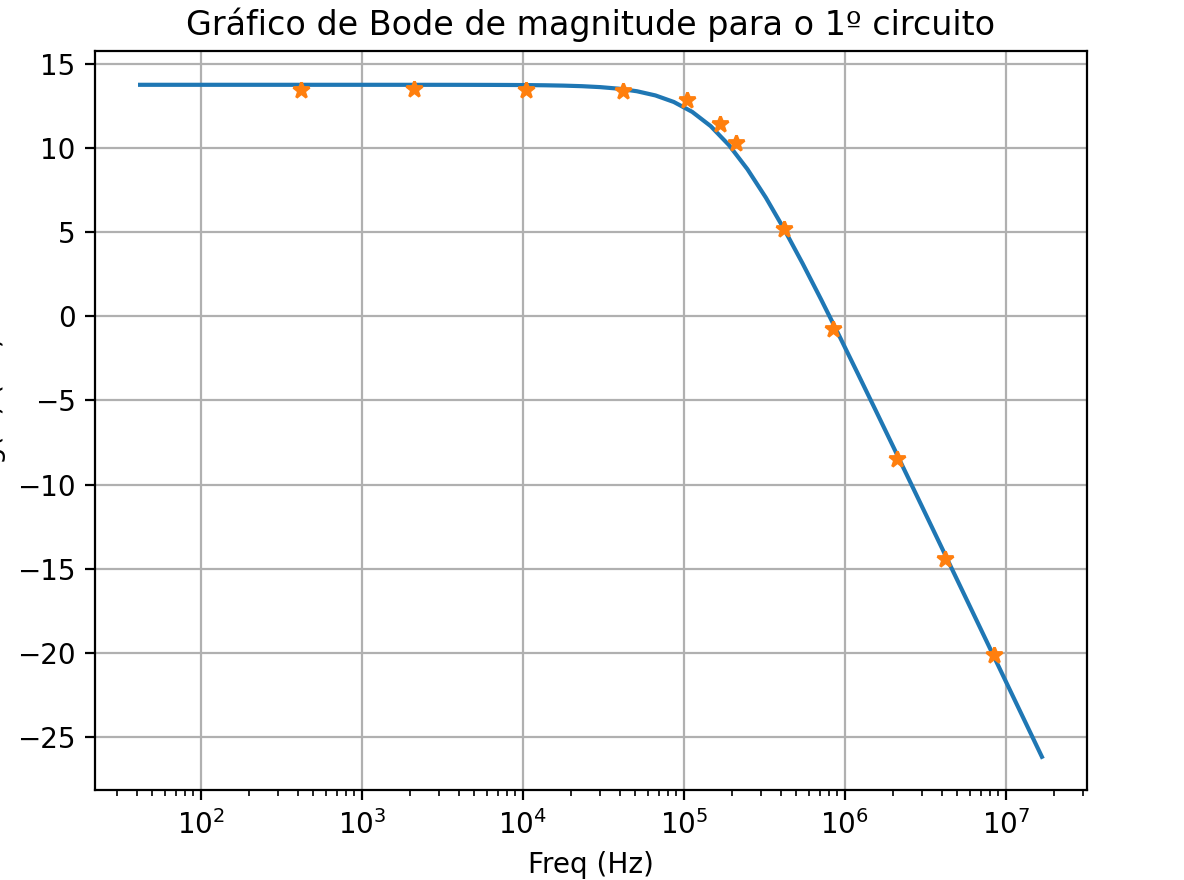
\includegraphics[width=1\columnwidth]{images/bode1.png}
    \caption{Gráfico de Bode para o primeiro circuito.}
\end{figure}

\newpage
\subsection{Circuito 2}


\subsubsection{Ajuste de curva}


Pelo código de ajuste de curva obtivemos os seguintes valores:


\begin{equation}
    \begin{aligned}
        K   & = -120.1                   \\
        f_c & =  9701.2 Hz = 60954 rad/s
    \end{aligned}
\end{equation}


Que são coerentes e próximos com os valores achados anteriormente na equação (9).


\subsubsection{Gráfico de Bode}


\begin{figure}[H]
    \centering
    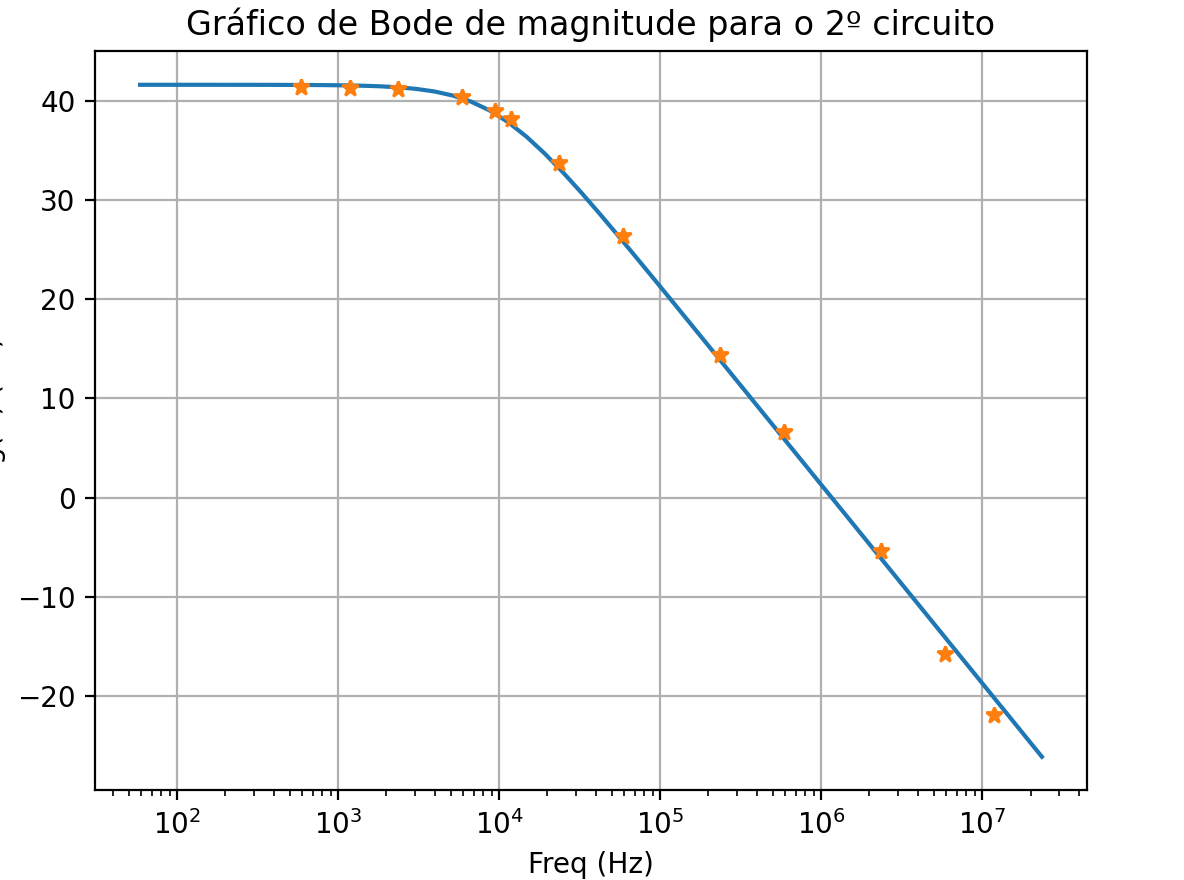
\includegraphics[width=1\columnwidth]{images/bode2.png}
    \caption{Gráfico de Bode para o segundo circuito.}
\end{figure}






\subsection{Gráfico de Bode de ambos circuitos.}


\begin{figure}[H]
    \centering
    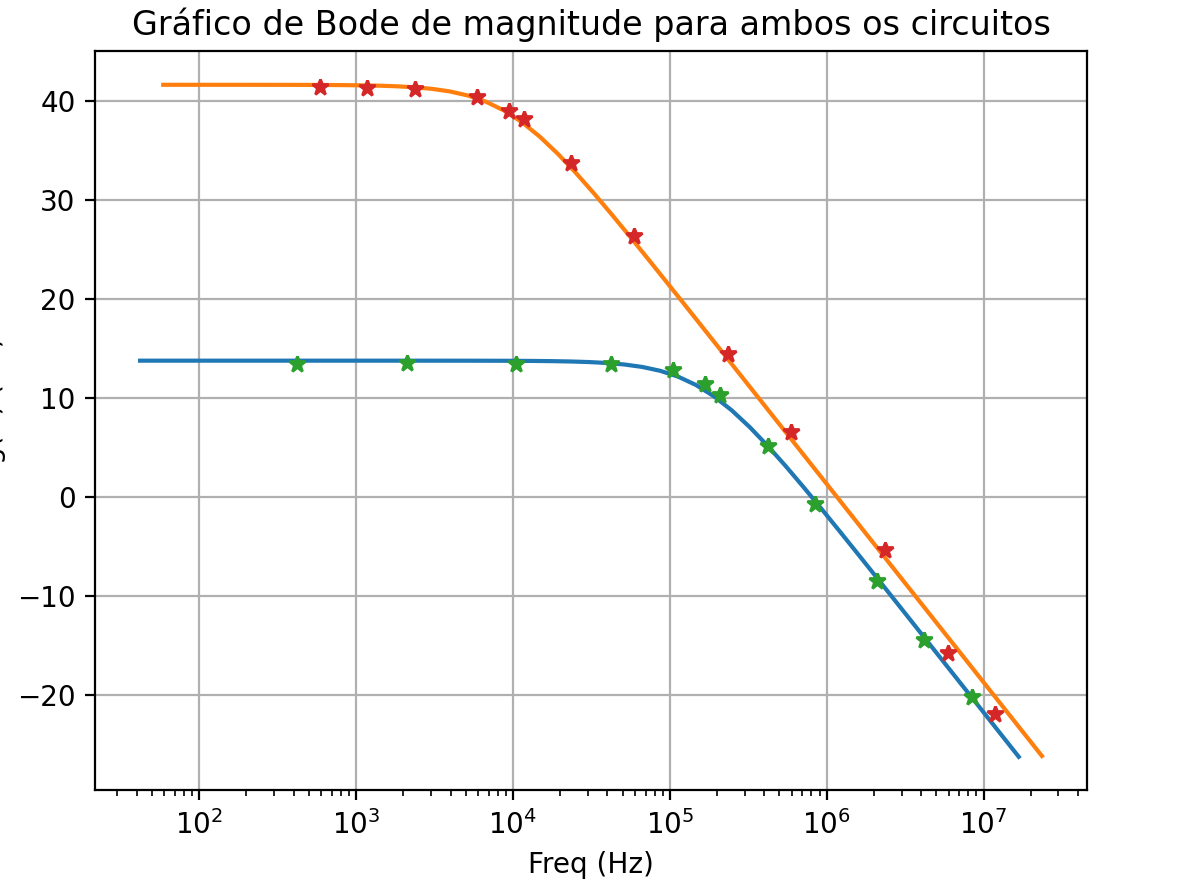
\includegraphics[width=1\columnwidth]{images/bodeboth.png}
    \caption{Gráfico de Bode para ambos circuitos sobrepostos.}
\end{figure}

